\documentclass{exam}

\usepackage{fullpage}
\usepackage{enumerate}
\usepackage{siunitx} 
\usepackage{graphicx}
\usepackage[fleqn]{amsmath}
\usepackage{cancel}
\usepackage{polynom}
\usepackage{float}
\usepackage{mdwlist}
\usepackage{booktabs}
\usepackage{cancel}
\usepackage{polynom}
\usepackage{caption}

\newcommand{\degree}{\ensuremath{^\circ}} 
\everymath{\displaystyle}

% \begin{figure}[H]
%   \centering
%   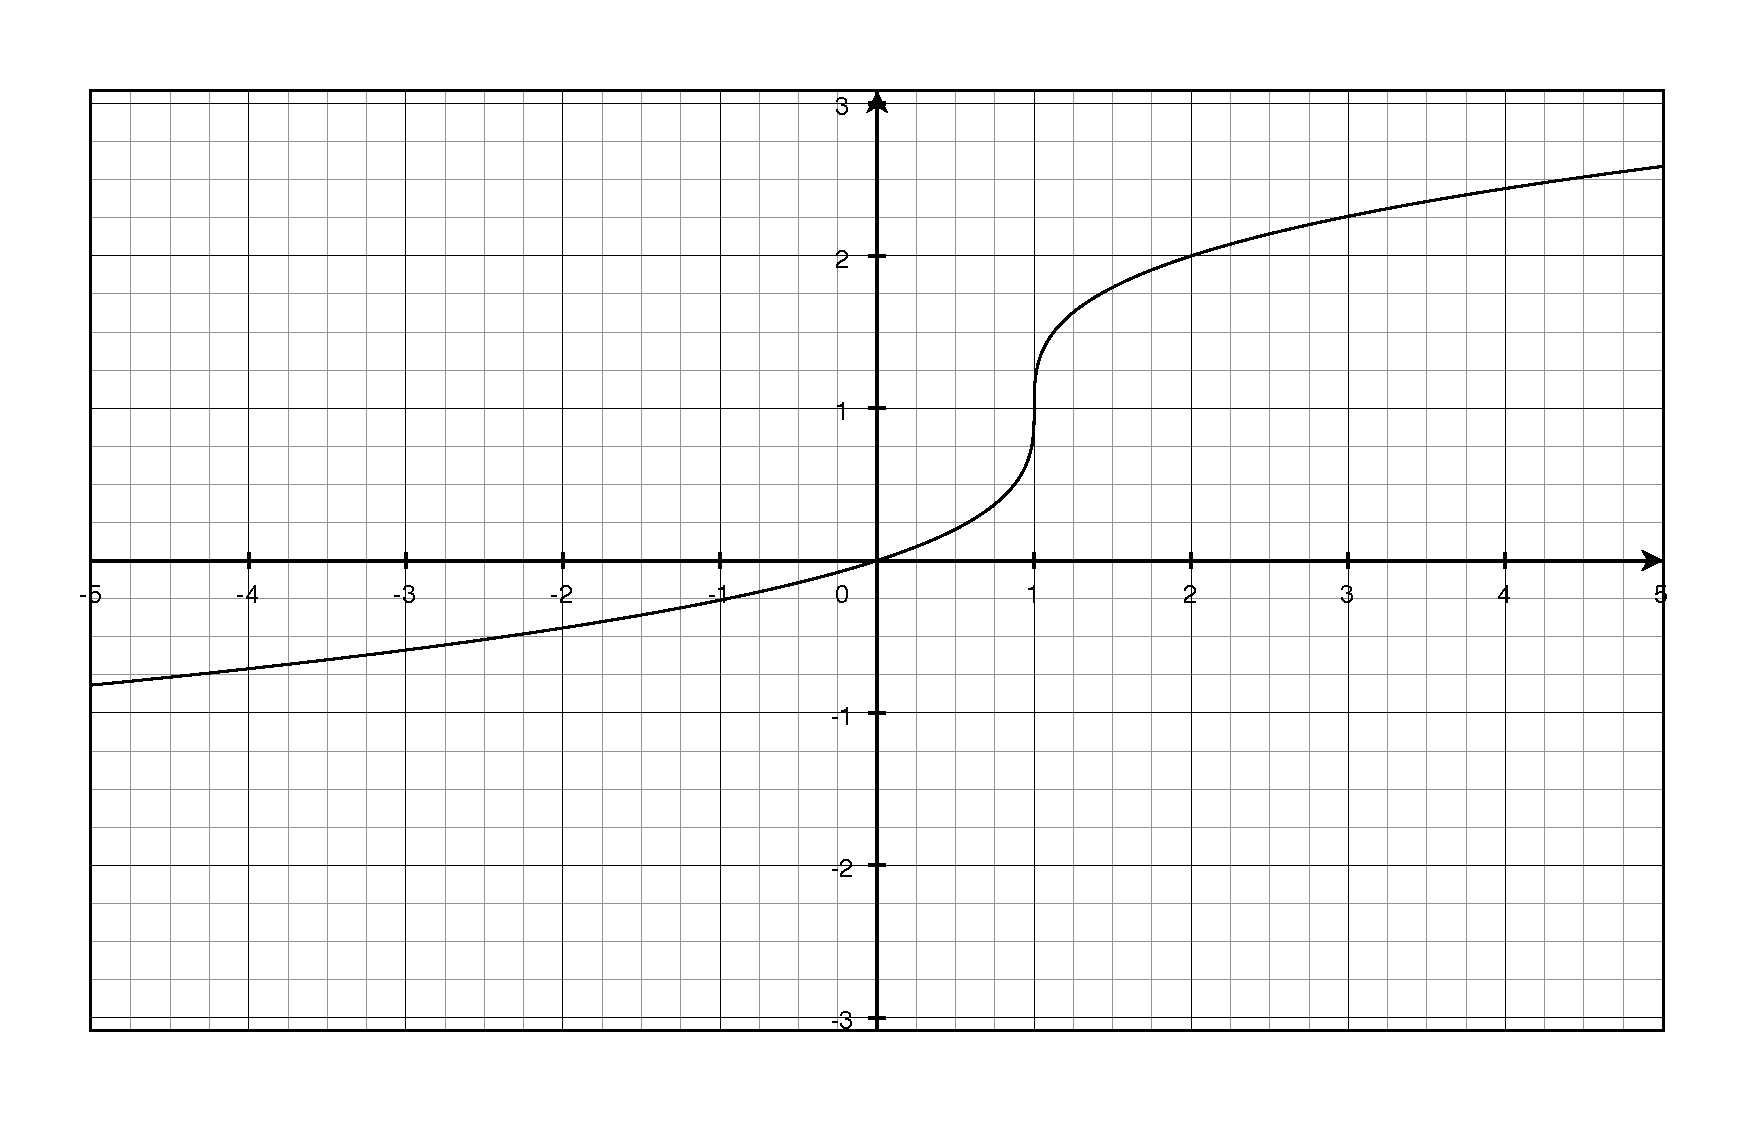
\includegraphics[scale=.3]{question7.eps}
%   \caption*{Question 7}
% \end{figure}

% \begin{tabular}{cc}
% \toprule
% period & amplitude \\
% \midrule
%   $\pi$ & $2$ \\
% \bottomrule
% \end{tabular}

\printanswers

\ifprintanswers 
\usepackage{2in1, lscape} 
\fi

\title{Math 263a \\ Homework 8}
\date{March 14, 2012 \\ Pi Day}

\begin{document}

\maketitle

\section{Homework}

\begin{itemize*}
  \item Read Section 3.6-3.7
  \item pp. 137-139: 16-25, 31
  \item pp. 145-146: 1-5, 11-15, 22, 26, 29, 32, 34
\end{itemize*}

\section{Extra Credit}
\begin{itemize*}
\item page 138, problem 34
\begin{solution}
If you draw a picture of the clock, you can see that the band is the hypotenuse of a triangle where one leg is 
$r \cos \theta$ and the other leg is $r - r \sin \theta$.  This means that the length of the band is:
\[
  b(\theta) = \sqrt{r^2 \cos^2 \theta + (1 - r \sin \theta)^2} = r \sqrt{2 - 2 \sin \theta}
\]

For a sanity check, you can check a few angles and find that the length of the band is 0 at 12:00, $r \sqrt{2}$ at 12:15
or 12:45 and $2r$ at 12:30, which all make sense.

We want an expression for the band length in terms of time, not in terms of $\theta$.  If we measure time in hours, the
angle is:
\[
  \theta = -2 \pi t
\]
The velocity of the hand is negative because clock hands move clockwise while angles increase in the counter-clockwise
direction.

So the expression for the length of the band in terms of time is:
\[
  b(t) = r \sqrt{2 - 2 \sin(- 2 \pi t) }
\]

Now we can find $\frac{db}{dt}$:
\begin{align*}
  \frac{db}{dt} &= \frac{d}{dt} (r \sqrt{2 - 2 \sin(-2 \pi t)}) \\
  &= r \frac{1}{2} (2 - 2 \sin (2 \pi \theta))^{-1/2} (-2 \cos (- 2 \pi \theta)) (-2 \pi) \\
  &= \frac{2 \pi r \cos (- 2 \pi \theta)}{\sqrt{2 - 2 \sin(- 2 \pi \theta)}} \\
\end{align*}

The numbers we're interested in are $\theta = 0$ and $r = 10$:
\[
  \frac{db}{dt} = \frac{20 \pi \cos 0}{\sqrt{2 - 2 \sin 0}} = \frac{20 \pi}{\sqrt{2}} = 10 \pi \sqrt{2} 
\]

This graph shows both the derivative of the length of the band and the length.

\begin{figure}[H]
  \centering
  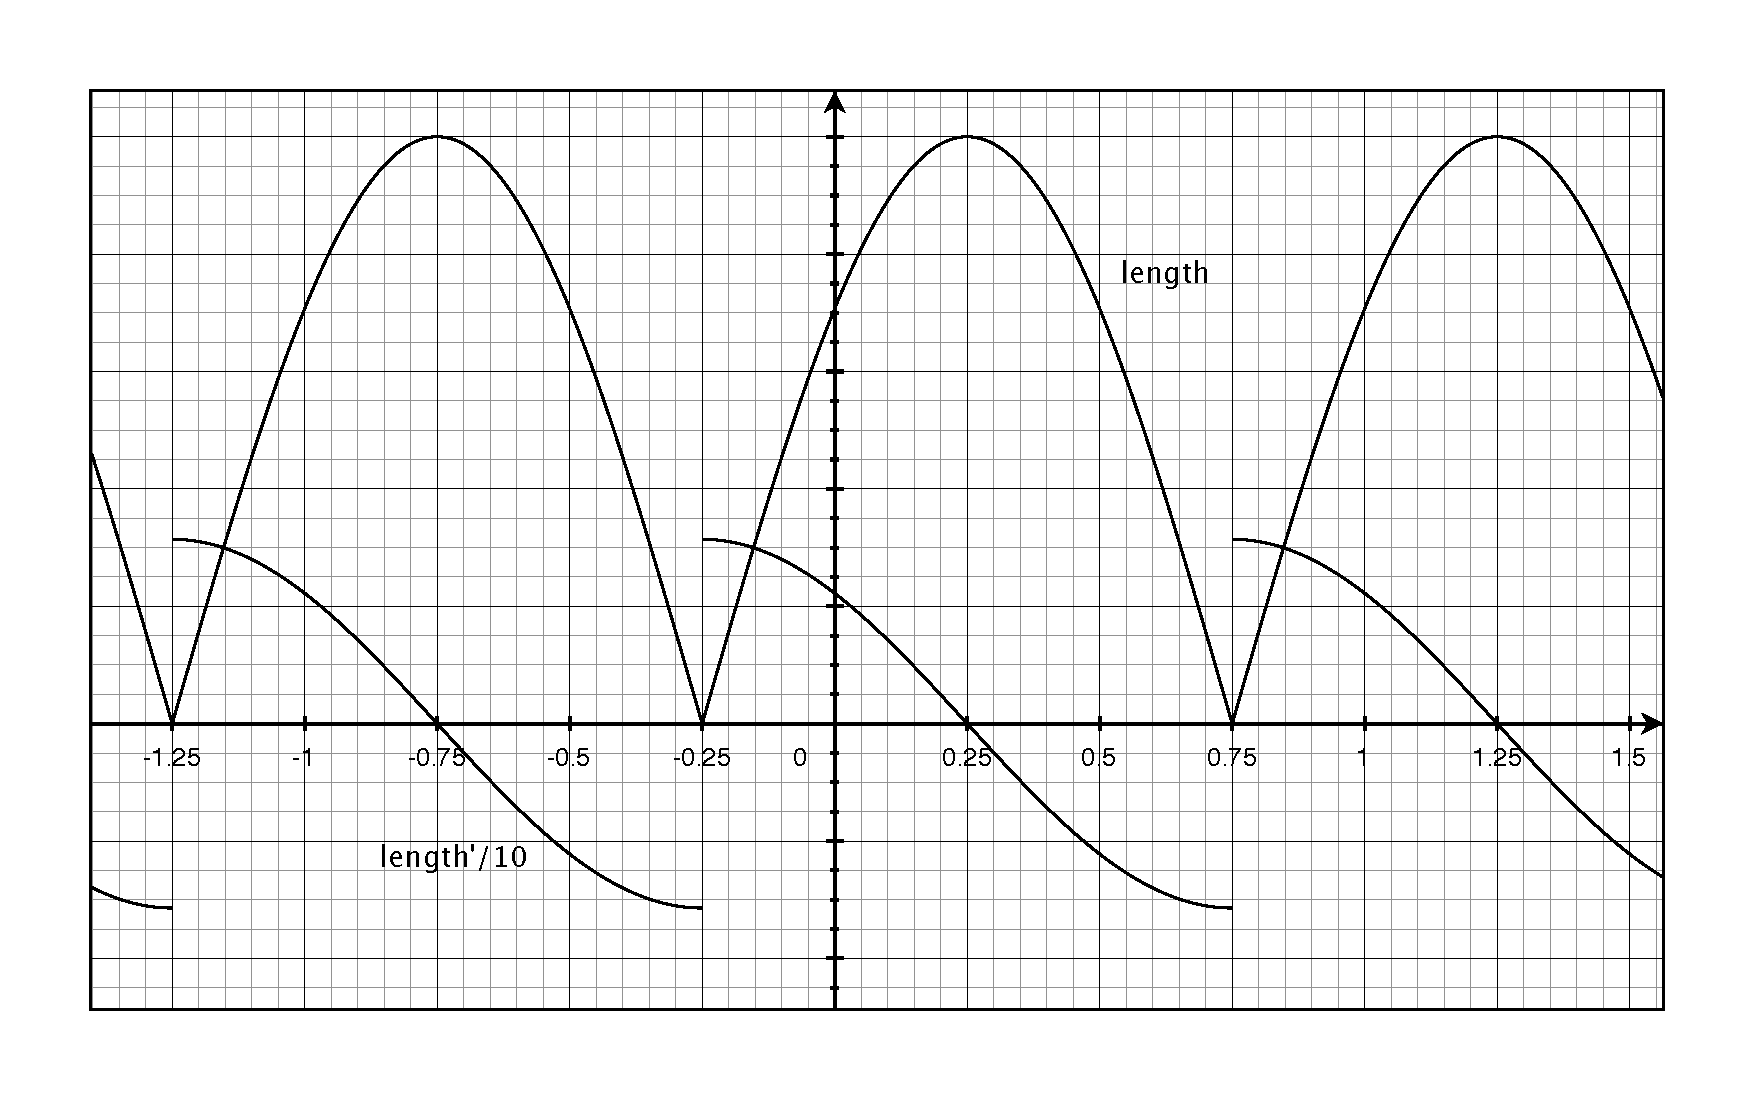
\includegraphics[scale=.3]{extra_credit_34.eps}
  \caption*{Clock Hands}
\end{figure}

There are some interesting things to notice:
\begin{itemize*}
\item The derivative is 0 when the band is stretched to its maximum point at 12:30.
\item The absolute value of the derivative is largest around 12:00.  This is when the length of the band is changing
  most rapidly.
\item The derivative jumps from a large positive value to a large negative value at 12:00.  This is when the band stop
  shrinking rapidly and starts stretching rapidly.
\item Because the hands on a clock go clockwise and angles are measured counter-clockwise, you need to read the graph
  from right to left if you want to see the normal progression of the clock hands.
\end{itemize*}

\end{solution}

\item page 145, problem 36
\begin{solution}
\begin{align*}
  s(t) &= v_0t + 16t^2 \\
  s'(t) &= v(t) = v_0 + 32t \\
\end{align*}

When it hits the ground after 3 seconds, its velocity is 140.  We can use this information to find the initial velocity.
\begin{align*}
  140 &= v_0 + 32 \cdot 3 \\
  v_0 &= 44 \text{ ft/s}\\
\end{align*}

Now we can use the initial velocity to find the height of the cliff:
\begin{align*}
  s(t) &= 44t + 16t^2 \\
  s &= 44 \cdot 3 + 16 \cdot 9 \\
    &= 276 \text{ ft}
\end{align*}


\end{solution}

\end{itemize*}

\ifprintanswers

\section{Homework}

\subsection{Section 3.6}

\begin{description}

% \item[15]
% \begin{align*}
%   y  &= \cos(x^2) \sin^2(x) \\
%   \frac{dy}{dx} &= \cos(x^2) \cdot 2 \sin(x) \cos(x) + \sin^2(x) \cdot [-\sin(x^2)(2x)] \\
%                 &= 2 \sin(x) \cos(x) \cos(x^2) - 2x \sin^2(x) \sin(x^2) \\
% \end{align*}

\item[16]
\begin{align*}
  y &= \frac{(x^3 + 2x)^4}{x^4 + 1} \\
  \frac{dy}{dx} &= \frac{(x^4 + 1) \cdot 4(x^3 + 2x)^3(3x^2 + 2) - (x^3 + 2x)^4(4x^3)}{(x^4 + 1)} \\
  &= \frac{ (x^3 + 2x)^3 [ (x^4 + 1)(12x^2 + 8) - (4x^6 + 8x^4) ]}{(x^4 + 1)^2} \\
  &= \frac{ (x^3 + 2x)^3 (12x^6 + 8x^4 + 12x^2 + 8 - 4x^6 - 8x^4)}{(x^4 + 1)^2} \\
  &= \frac{ (x^3 + 2x)^3 (8x^6 + 12x^2 + 8 )}{(x^4 + 1)^2} \\
\end{align*}

\item[17]
\begin{align*}
  y  &= \sin^4(x^2 + 3) \\
  \frac{dy}{dx} &= 8x \sin^3(x_2 + 3) \cos(x^2 + 3) \\
\end{align*}

\item[18]
\begin{align*}
  y &= \sin [ (x^2 + 3)^4] \\
  \frac{dy}{dx} &= \cos [ (x^2 + 3)^4] \cdot 4(x^2 + 3)^3 \cdot 2x \\
                &= 8x (x^2 + 3)^3 \cos [ (x^2 + 3)^4]  \\
\end{align*}

\item[19]
\begin{align*}
  y &= \cos^2 \left( \frac{x^2 + 2}{x^2 - 2} \right) \\
  \frac{dy}{dx} &= 2 \cos \left( \frac{x^2 + 2}{x^2 - 2} \right) 
    \cdot \left[ - \sin \left( \frac{x^2 + 2}{x^2 - 2} \right) \right] 
    \cdot \frac{2x^3 - 4x - (2x^3 + 4x)}{(x^2 - 2)^2} \\
  &= -2 \cos \left( \frac{x^2 + 2}{x^2 - 2} \right) 
    \sin \left( \frac{x^2 + 2}{x^2 - 2} \right) 
    \cdot \frac{2x^3 - 4x - 2x^3 - 4x}{(x^2 - 2)^2} \\
  &= \cos \left( \frac{x^2 + 2}{x^2 - 2} \right) 
     \sin \left( \frac{x^2 + 2}{x^2 - 2} \right) 
     \cdot \frac{16x}{(x^2 - 2)^2} \\
\end{align*}

\item[20]
\begin{align*}
  y &= \sin^2 [ \cos^2 (x^2) ] \\
  \frac{dy}{dx} &= 2 \sin [ \cos^2 (x^2) ] \cdot \cos [ \cos^2 (x^2) ] \cdot 2 \cos (x^2) \cdot (- \sin(x^2)) \cdot 2x \\
   &= -8x \cdot \sin [ \cos^2 (x^2) ] \cdot \cos [ \cos^2 (x^2) ] \cdot \cos (x^2) \cdot \sin(x^2)  \\
\end{align*}

\item[21]
\begin{align*}
  \frac{d}{dt} (\sin^3 t + \cos^3 t) &= 3 \sin^2 t \cos t - 3 \cos^2 t \sin t \\
\end{align*}

\item[22]
\begin{align*}
  \frac{d}{ds} [ (s^2 + 3)^3 &- (s^2 + 3)^{-3} ] = 3 (s^2 + 3)^2(2s) - (-3)(s^2 + 3)^{-4}(2s) \\
    &= 6s (s^2 + 3)^2 + 6s (s^2 + 3)^{-4} \\
    &= 6s [ (s^2 + 3)^2 + (s^2 + 3)^{-4} ] \\
\end{align*}

\item[23]
\begin{align*}
  D_x [ & \pi (r + 3)^2 - 3 \pi r (r + 2)^2 ] \\
    &=  \pi D_x [ (r + 3)^2 - 3 r (r + 2)^2 ] \\
    &= \pi [ 2 (r + 3) - [ 3 r \cdot 2(r + 2) + (r + 2)^2 \cdot 3] ] \\
    &= \pi [ 2r + 6 - 6r(r + 2) - 3(r^2 + 4r + 4)] \\
    &= \pi [ 2r + 6 - 6r^2 - 12r - 3r^2 - 12r - 12] \\
    &= -9 \pi r^2 - 22 \pi r - 6 \pi \\
\end{align*}

\item[24]
\begin{align*}
  D_t [ t^6 + 3t^2 ] &= 6t^5 + 6t
\end{align*}

\item[25]
\begin{align*}
  f(x) &= ( x + x^{-1} )^4 \\
  f'(x) &= 4(x + x^{-1})^3 (1 - x^{-2}) \\
        &= 4 \left(x + \frac{1}{x} \right)^3 \left(1 - \frac{1}{x^2} \right) \\
  f'(2) &= 4 \left(2 + \frac{1}{2} \right)^3 \left(1 - \frac{1}{4} \right) \\
        &= 4 \left(\frac{5}{2} \right)^3 \left(\frac{3}{4} \right) \\
        &= \frac{375}{8}  \\
\end{align*}

\item[31]
\begin{enumerate}[a]

\item
\begin{align*}
  v &= x^3 \\ 
  \frac{dv}{dt} &= 3x^2 \cdot \frac{dx}{dt} \\  
\end{align*}

when $x = 20$:
\[
  \frac{dv}{dt} = 3 \cdot (20^2) \cdot 16 = 19,200 \cm^3 \per \min \\  
\]

\item
\begin{align*}
  A &= 6 x^2 \\ 
  \frac{dA}{dt} &= 12x \cdot \frac{dx}{dt} \\  
\end{align*}

when $x = 15$:
\[
  \frac{dA}{dt} = 12 \cdot 15 \cdot 16 = 2,880 \cm^2 \per \min \\  
\]

\end{enumerate}

\end{description}

\subsection{Section 3.7}

\begin{description}
\item[1]
\begin{align*}
  y &= x^3 + 3x^2 + 6x \\
  \frac{dy}{dx} &= 3x^2 + 6x + 6 \\
  \frac{d^2y}{dx^2} &= 6x + 6 \\
  \frac{d^3y}{dx^3} &= 6 \\
\end{align*}

\item[2]
\begin{align*}
  y &= x^5 + x^4 \\
  \frac{dy}{dx} &= 5x^4 + 4x^3 \\
  \frac{d^2y}{dx^2} &= 20x^3 + 12x^2 \\
  \frac{d^3y}{dx^3} &= 60x^2 + 24x \\
\end{align*}

\item[3]
\begin{align*}
  y &= (3x + 5)^3 \\
  \frac{dy}{dx} &= 3(3x + 5)^2 \cdot 3 = 9(3x+5)^2 \\
  \frac{d^2y}{dx^2} &= 9 \cdot 2 (3x+5) \cdot 3 = 54(3x+5) \\
  \frac{d^3y}{dx^3} &= 54 \cdot 3 = 162 \\
\end{align*}

\item[4]
\begin{align*}
  y &= (3 - 5x)^5 \\
  \frac{dy}{dx} &= 5(3 - 5x)^4 \cdot (-5) = -25 (3 - 5x)^4 \\
  \frac{d^2y}{dx^2} &= -100 (3 - 5x)^3(-5) = 500(3 - 5x)^3 \\
  \frac{d^3y}{dx^3} &= 1,500 (3 - 5x)^2 (-5) = -7,500 (3 - 5x)^2 \\
\end{align*}

\item[5]
\begin{align*}
  y &= \sin(7x) \\
  \frac{dy}{dx} &= 7 \cos(7x) \\
  \frac{d^2y}{dx^2} &= -49 \sin(7x) \\
  \frac{d^3y}{dx^3} &= -343 \cos(7x) \\
\end{align*}

\item[11]
\begin{align*}
  f(t)   &= 2t^{-1} \\
  f'(t)  &= -2t^{-2} \\
  f''(t) &= 4t^{-3} = \frac{4}{t^3} \\
  f''(2) &= \frac{4}{2^3} = \frac{1}{2} \\ 
\end{align*}

\item[12]
\begin{align*}
  f(u)   &=  \frac{2u^2}{5-u} \\
  f'(u)  &=  \frac{(5-u)(4u) - (2u^2)(-1)}{(5-u)^2} \\
         &=  \frac{20u -4u^2 + 2u^2}{(5-u)^2} \\
         &=  \frac{20u - 2u^2}{(5-u)^2} \\
  f''(u) &=  \frac{(5-u)^2(20-4u) - (20u - 2u^2)(2)(5-u)(-1)}{(5-u)^4} \\
         &=  \frac{(5-u)(20-4u) + 2(20u - 2u^2)}{(5-u)^3} \\
         &=  \frac{100 - 40u + 4u^2 + 40u - 4u^2}{(5-u)^3} \\
         &=  \frac{100}{(5-u)^3} \\
  f''(2) &=  \frac{100}{(5-2)^3} = \frac{100}{27} \\
\end{align*}

\item[13]
\begin{align*}
  f(\theta)   &= (\cos \pi \theta)^{-2} \\
  f'(\theta)  &= -2 \pi \cdot (\cos \pi \theta)^{-3} \sin \pi \theta \\
  f''(\theta) &= 2 \pi [ (\cos \pi \theta)^{-3}(\cos \pi \theta)(\pi) + (\sin \pi \theta)(-3)(\cos \pi \theta)^{-4}(- \sin \pi \theta)(\pi) \\
              &= 2 \pi^2 \left[ \sec^2 \pi \theta + \frac{3 \sin^2 \pi \theta}{\cos^4 \pi \theta} \right] \\
              &= 2 \pi^2 \left[ \sec^2 \pi \theta + 3 \tan^2 \pi \theta \sec^2 \pi \theta \right] \\
  f''(2)      &= 2 \pi^2 \\
\end{align*}

\item[14]
\begin{align*}
  f(t)   &= t \sin(\pi t^{-1}) \\
  f'(t)  &= - \pi t^{-1} \cos(\pi t^{-1}) + \sin(\pi t^{-1}) \\
  f''(t) &= - \pi t^{-1} [- \sin(\pi t^{-1})] (- \pi t^{-2}) + \cos(\pi t^{-1})(\pi t^{-2}) + \cos(\pi t^{-1}) (- \pi t^{-2}) \\
         &= - \frac{\pi^2}{t^3} \sin \frac{\pi}{t} \\
  f''(2) &= - \frac{\pi^2}{8} \\  
\end{align*}

\item[15]
\begin{align*}
  f(t)   &= s(1-s^2)^3 \\
         &= -s^7 + 3s^5 - 3s^3 + s \\
  f'(t)  &= -7s^6 + 15s^4 - 9s^2 + 1 \\
  f''(t) &= -42s^5 + 60s^3 - 18s \\
  f''(2) &= -900 \\ 
\end{align*}

\item[22]
\begin{align*}
  g(t)   &= at^2 + bt + c \\
  g'(t)  &= 2at + b \\
  g''(t) &= 2a \\
  \\ 
  -4 &= 2a \\
  a  &= -2 \\
  \\
  3 &= -4 + b \\
  b &= 7 \\
  \\
  5 &= -2 + 7 + c\\
  c &= 0 \\
\end{align*}

The equation is: $g(t) = -2t^2 + 7t$

\item[26]
\[
  s = 2t^3 - 6t + 5
\]

\begin{enumerate}[a]
\item
\begin{align*}
  v &= 6t^2 - 6 \\
  a &= 12 t \\
\end{align*}

\item
The object is moving right when the velocity is positive:
\begin{align*}
  6t^2 - 6 &> 0 \\
  t^2 &> 1 \\
  t < -1 & \text{ or } t > 1 \\
\end{align*}

\item
The object is moving left when $-1 < t < 1$.

\item
\begin{align*}
  12t < 0 \\
  t < 0 \\
\end{align*}

\end{enumerate}

\item[29]
\begin{align*}
  s &= \frac{1}{2}t^4 - 5t^3 + 12t^2 \\
  v &= 2t^3 - 15t^2 + 24t \\
  a &= 6t^2 - 30t + 24 \\
\end{align*}
\begin{align*}
  6t^2 - 30t + 24 &= 0 \\
  t^2 - 5t + 4 &= 0 \\
  (t-4)(t-1) &= 0 \\
\end{align*}

$t = \{1, 4\}$; $v(1) = 11$, $v(4) = -16$

\item[32]
\begin{align*}
  s_1 &= 3t^3 - 12t^2 + 18t + 5 \\
  s_1' &= 9t^2 - 12t + 18 \\
  \\
  s_2 &= -t^3 + 9t^2 - 12t \\
  s_2' &= -3t^2 + 18t - 12 \\
\end{align*}

\begin{align*}
  9t^2 - 12t + 18 &= -3t^2 + 18t - 12 \\
  2t^2 - 7t + 5 &= 0 \\
  (2t - 5)(t - 1) &= 0 \\
\end{align*}

$t = \left\{\frac{5}{2}, 1\right\}$

\item[34]
\begin{align*}
  s &= 48t - 16t^2 \\
  v &= 48 - 32t \\
\end{align*}


\begin{enumerate}[a]

\item
The maximum height is reached when the velocity is zero:
\begin{align*}
  48 - 32t &= 0 \\
  t &= \frac{3}{2} \\
\end{align*}

\item
After 1 second:
\[
  v(1) = 48 - 32 = 16 \\
\]
Since the volume is positive, the object is still moving up since the velocity is positive.

The object gets back to zero when:
\begin{align*}
  48t - 16t^2 &= 0 \\
  t(3-t) &= 0 \\
\end{align*}

The object is on the ground when it starts out at 0 seconds and when it falls back after its trip at 3 seconds.

\end{enumerate}

\end{description}


\else

\vspace{8 cm}

{\em If you go to the city of Washington, and you examine the pages of the Congressional Directory, you will find that
  almost all of those corporation lawyers and cowardly politicians, members of Congress, and misrepresentatives of the
  masses---you will find that almost all of them claim, in glowing terms, that they have risen from the ranks to places
  of eminence and distinction. I am very glad I cannot make that claim for myself. I would be ashamed to admit that I
  had risen from the ranks. When I rise it will be with the ranks, and not from the ranks.}

\vspace{.2 cm}

\hspace{1 cm} --Eugene V. Debs

% for approximation {\em From this point forth we shall be leaving the firm foundation of fact and journeying together
% through the murcky marshes of memory into thickets of wildest guesswork.} (Dumbledore)(Can be used right in front of
% the Humphrey Belcher quote if desired. From page 197. Humphrey Belcher quote is also from page 197. Harry Potter and
% the Half-Blood Prince. I love typing on this thing.

\fi

\end{document}

